\documentclass[letterpaper, 10pt,titlepage]{article}

\usepackage{graphicx} 
\graphicspath{ {images/} }                                       
\usepackage{amssymb}                                         
\usepackage{amsmath}                                         
\usepackage{amsthm}                                          
\usepackage{alltt}                                           
\usepackage{float}
\usepackage{color}
\usepackage{url}
\usepackage[letterpaper, margin=0.75in]{geometry}
\usepackage{enumitem}
\usepackage{pstricks, pst-node}
\usepackage{hyperref}
\usepackage[utf8]{inputenc}
\usepackage{underscore}
 \usepackage{url}
\hypersetup{
  colorlinks = true,
  linkcolor  = black
}

\setcounter{secnumdepth}{4}
\def\name{Chongxian Chen}

\hypersetup{
  colorlinks = true,
  urlcolor = black,
  pdfauthor = {\name},
  pdfkeywords = {Problem Statement},
  pdftitle = {Capstone Project},
  pdfsubject = {Capstone Project},
  pdfpagemode = UseNone
}

\renewcommand*\contentsname{Table of Contents}


\begin{document}

\begin{center}

Oregon State University Computer Science Senior Design Winter 2016
\bigbreak
Progress Report
\bigbreak
By Alex Hoffer, Jake Smith, and Chen Chongxian
\bigbreak
Team Name: Stat Champs
\bigbreak
\vspace{3.0cm}
Abstract
\bigbreak
The application of machine learning to Biochemistry and Biophysics has enabled researchers in this field to make remarkable discoveries, such as the generation of new DNA sequences. However, students of Biochemistry and Biophysics do not get the opportunity to learn machine learning. Dr. Victor Hsu of the Oregon State University Biochemistry and Biophysics department has commissioned the Stat Champs to produce an instructional module to give his students the chance to familiarize themselves with machine learning. The software product the Stats Champs have agreed to develop is a web page that allows students to train a machine learning model based on the college basketball statistics and machine learning algorithm of their choosing in order to produce a March Madness bracket. This will help students understand how machine learning algorithms produce models and how inclusion or exclusion of certain data can influence such models. Over the course of Fall term 2016, the Stat Champs developed materials such as design documents and technology reviews in order to prepare for the engineering of the module. Then, in Winter term 2017, the Stat Champs began the software development phase of this project. This report comprehensively describes the progress thus made on this project, as of mid-February 2017.
\newpage
\end{center}

\tableofcontents

\newpage
\section{Introduction}
	This report chronicles the progress the Stat Champs have made on developing the machine learning instructional tool. In Fall term 2016, the progress that had been made was a project statement, a requirements document, a design document, a technology review, and a progress report. In Winter term 2017, the team made progress on the engineering of the module. The remaining sections of this report are devoted to each of the individual members of the Stat Champs to describe their experiences this term as well as their contributions to the software product.
\section{Progress Descriptions}
\subsection{Alex Hoffer}

\subsubsection{Project Purposes and Goals}
\par Our project was given to us by Dr. Victor Hsu of the Biochemistry and Biophysics department at Oregon State University. The purpose of this project is to demonstrate to Dr. Hsu's students how common machine learning algorithms generate models, and how the inclusion or exclusion of data can influence these models. Using an event like the March Madness tournament that produces binary outcomes (i.e. each team can only win or lose) facilitates the learning process by making the machine learned models easy to read, understand, and manipulate through the inclusion or exclusion of data. Thus, our goal is to help Dr. Hsu's students learn how machine learning works, and the degree to which our module is successful is predicted by whether or not the average student can begin to understand machine learning through our demonstration. 

\subsubsection{Brief recap of Alex's responsibilities}
\par As a team, we discussed each of our three responsibilities in Fall term 2016. My three responsibilities center around the graphical user interface (hereafter referred to as GUI) of the module. For me, the first responsibility was to host the web page and develop the general GUI to aid users in navigating the various sections of the website. Information pertaining to this first responsibility can be found in the subsection "Responsibility 1". Responsibility two was to present instructions on how to use the module before the machine learning module itself was presented. I have expanded this responsibility to include the development of two additional subsections of the site. These two additional, unplanned subsections are a Purpose page and an About page. These pages will be described in detail in the subsection "Responsibility 2", and my additions to my original second responsibility will be noted in a modified Technology Review document for the purpose of project documentation. My third responsibility was to take the data generated by Chongxian's machine learning algorithms and produce a March Madness bracket. More on the progress on this responsibility can be found in the section "Where Alex is Currently At in the Project". 
   
\subsubsection{Responsibility 1}
\par My first responsibility was to host the web page and develop the GUI for the project so that users can navigate through the website. Specifically, this responsibility consisted of four tasks. First, I hosted the website on my public_html folder that is provided to me by the Engineering department. Then, I had to produce HTML. That is, I had to construct the blueprints for what the site should look like. This consisted of things like a banner that contained links to different parts of the site, such as Home, Instructions, Module, Purpose, and About. Other than the banner, I added a title for the page to appear in the browser, the use of HTML divs, lists, sections, and other common tags to organize our website, which is just one big page, into logical chunks that correspond to the different features our website offers. While I established the parts of the site like Home, Instructions, etc., it was not until the second responsibility (which has its own section of this report dedicated to it) that I modified these in any way. My next task of this first responsibility was to produce CSS. Since my main motive in my contributions to this project were to ensure the usability of the module, it is only natural that I used CSS to customize the HTML tags. Without CSS, a website looks ugly. I added CSS that I believed would improve the user's experience with the website, because I felt that without a clean, readable interface, there would be unnecessary difficulties within the usage of the site that would hamper our target population's ability to learn machine learning. In other words, the hardest part to understand about this module should be the machine learning algorithms themselves, not the design that leads to using the module. The third task within this responsibility was to produce JavaScript. Without JavaScript, this page would be clunky and unresponsive. All moderately usable websites in our current era utilize JavaScript to make pages fun to use and to reduce the need for users to re-load the website to experience all features of the page, which serendipitiously also reduces the demand on the Engineering server the site is hosted on, which means more users can access our website at once. The specifics of the JavaScript contribution include making the individual items on the banner mentioned above light up when a mouse hovers over them, which helps keep the user informed about where they are in the web page. These list items located on the banner were also clickable, and when clicked, lead to the specific section of the page which its title referred to. This design decision was yet another opportunity to improve page usability by providing an intuitive way for users to navigate through the site, as well as reducing the load on the server by requiring fewer page refreshes. Therefore, the three technologies I required to fully implement this first responsibility were HTML, CSS, and JavaScript. The only problems I encountered in using these three technologies came from JavaScript, which I find to be a perplexing and complicated language. The use of JavaScript tutorials, programmer message boards, and documentation eased my woes in this dimension and enabled me to produce a GUI for our website that looks clean and understandable and is rewarding to interact with.
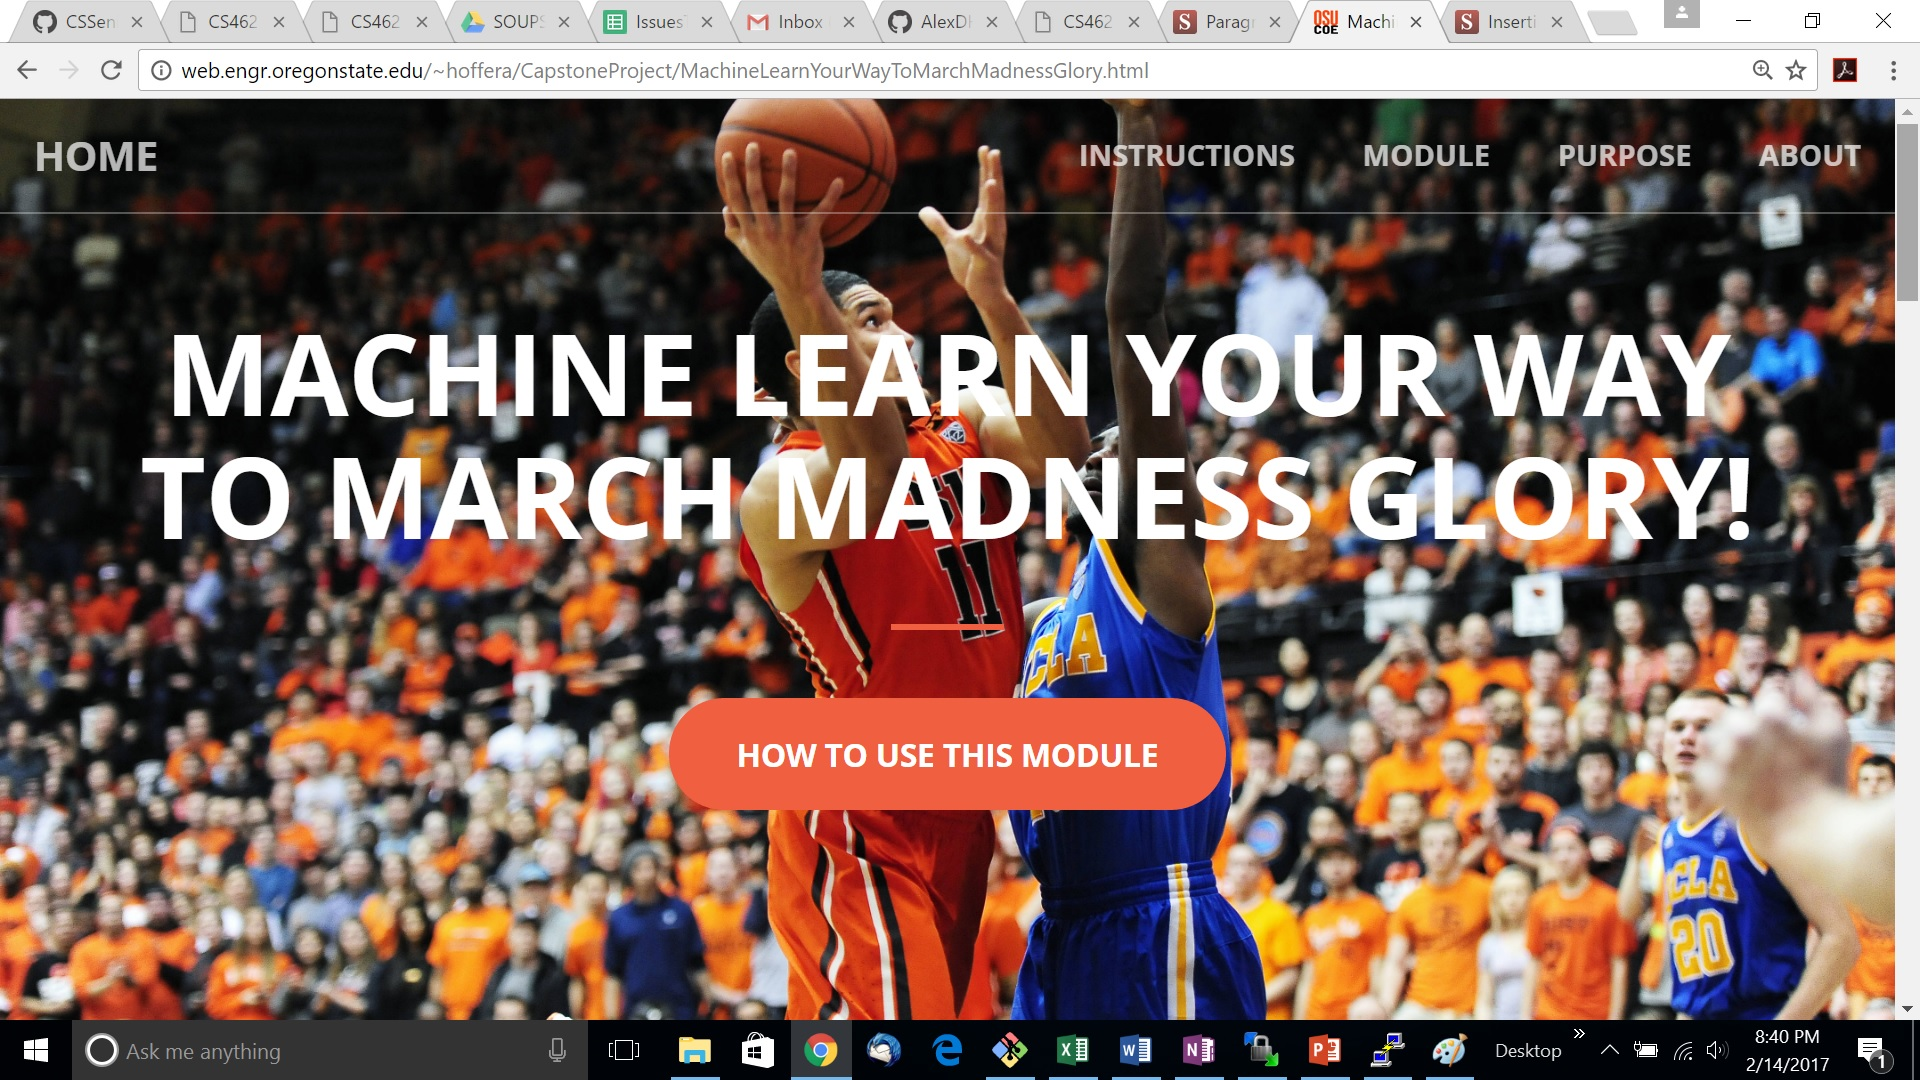
\includegraphics[width=\textwidth]{dv.jpg}
A screenshot image of the home page of our website. Images of each other section of the page can be found in the "Responsibility 2" section.

\subsubsection{Responsibility 2}
My second responsibility was to present instructions to the user on how to use the module before the module itself is presented. However, I expanded this responsibility after I developed the GUI in my first responsibility to encompass not only a section of the page devoted to the instructions, but also sections devoted to our purpose, about us, and the module itself. The instructions are thus far incomplete because we have not been able to get our machine learning module working (the responsibilities for the machine learning module functionality lie within other group mates' sections). There is currently a section of the page devoted to the module itself, which is also, given the incomplete status of the module, not occupied by anything meaningful. However, I have written the Purpose section (which encapsulates descriptions of this project's purpose that can be read in my section "Project Purposes and Goals", as well as the About Us section, which simply describes who we are and how to reach us if need be. The development of these sections was easy, since I merely built upon the GUI that I developed in my first responsibility. Therefore, through the combined magic of CSS and JavaScript I was able to produce a clean interface for all of these sections of our website. A particularly nice feature of note that was made possible by these two technologies is a button located at the bottom of each section that lit up when a mouse hovered over it and, if clicked, bounced the user on down to the next logical section of the website. The content of these sections can be found in images presented below.

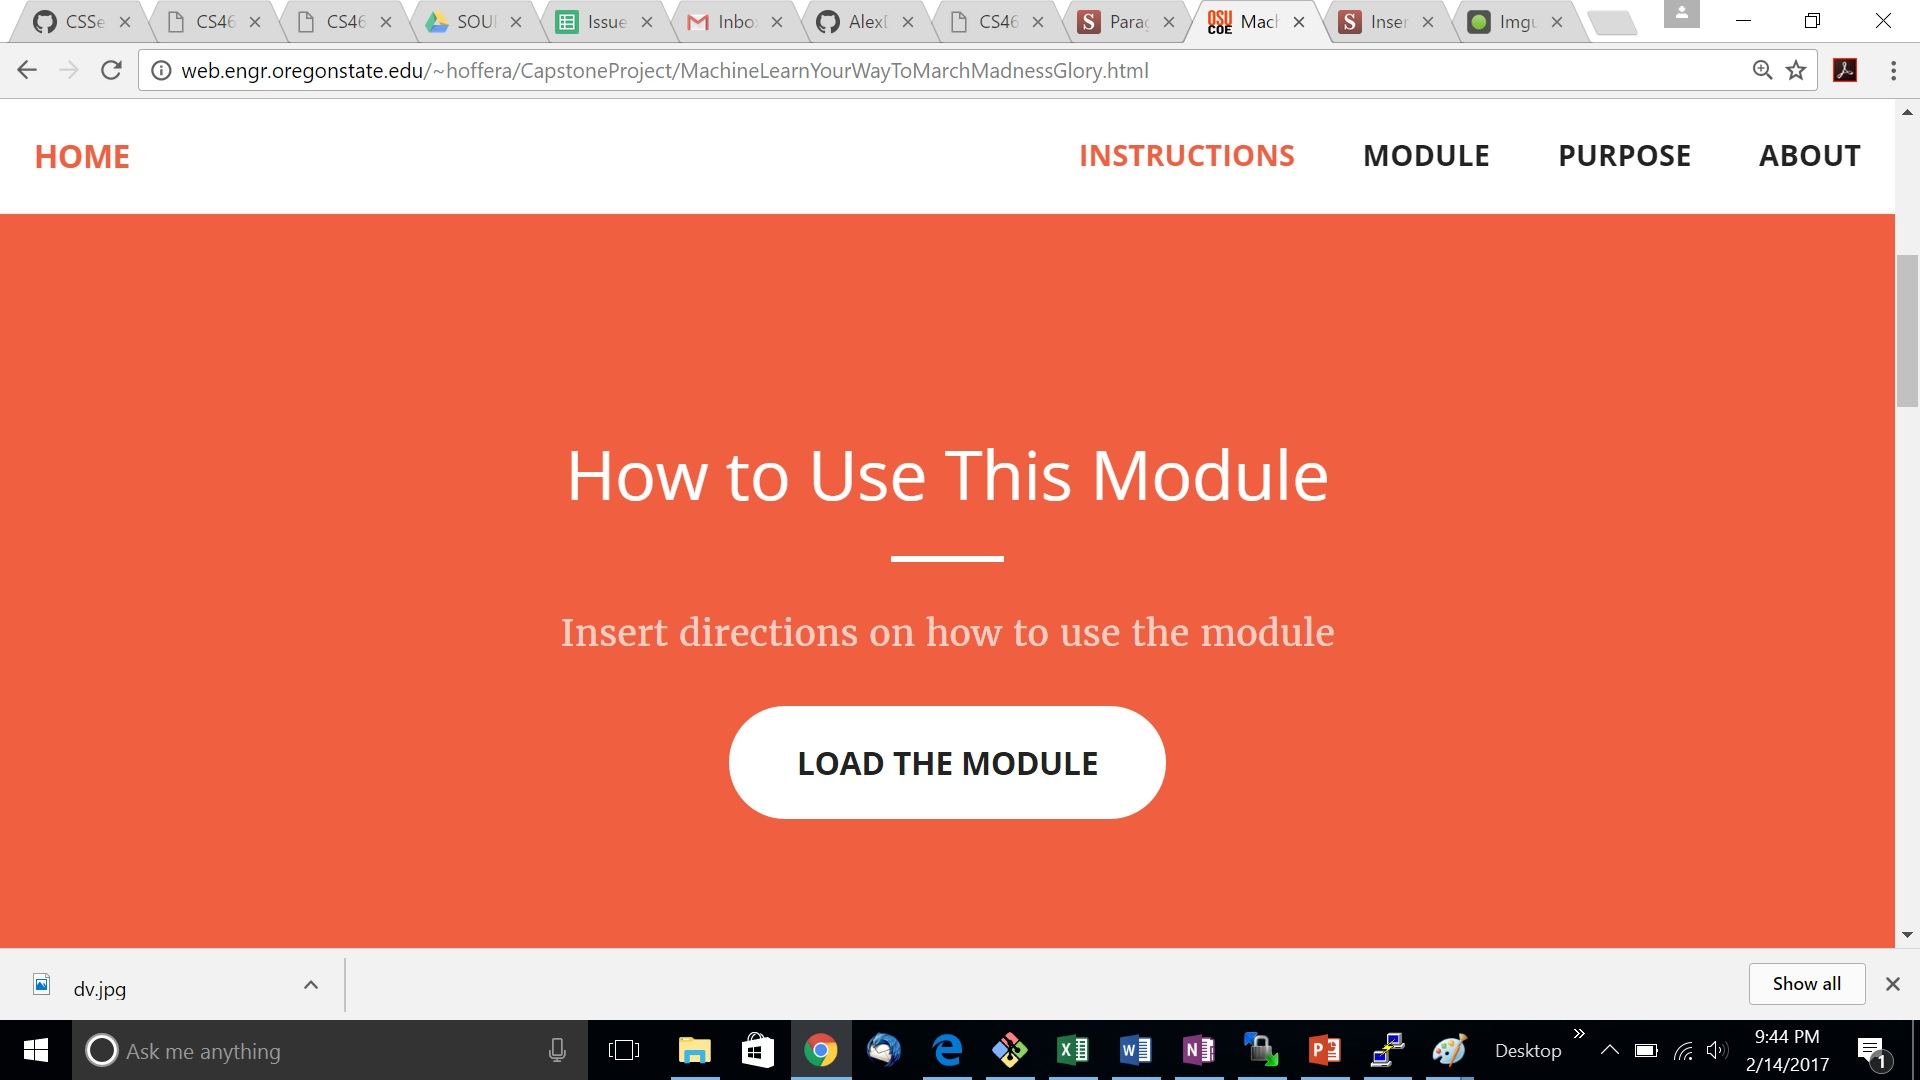
\includegraphics[width=\textwidth]{Instructions.jpg}
A screenshot image of the Instructions page of our website. Note that it remains incomplete until the module is created.

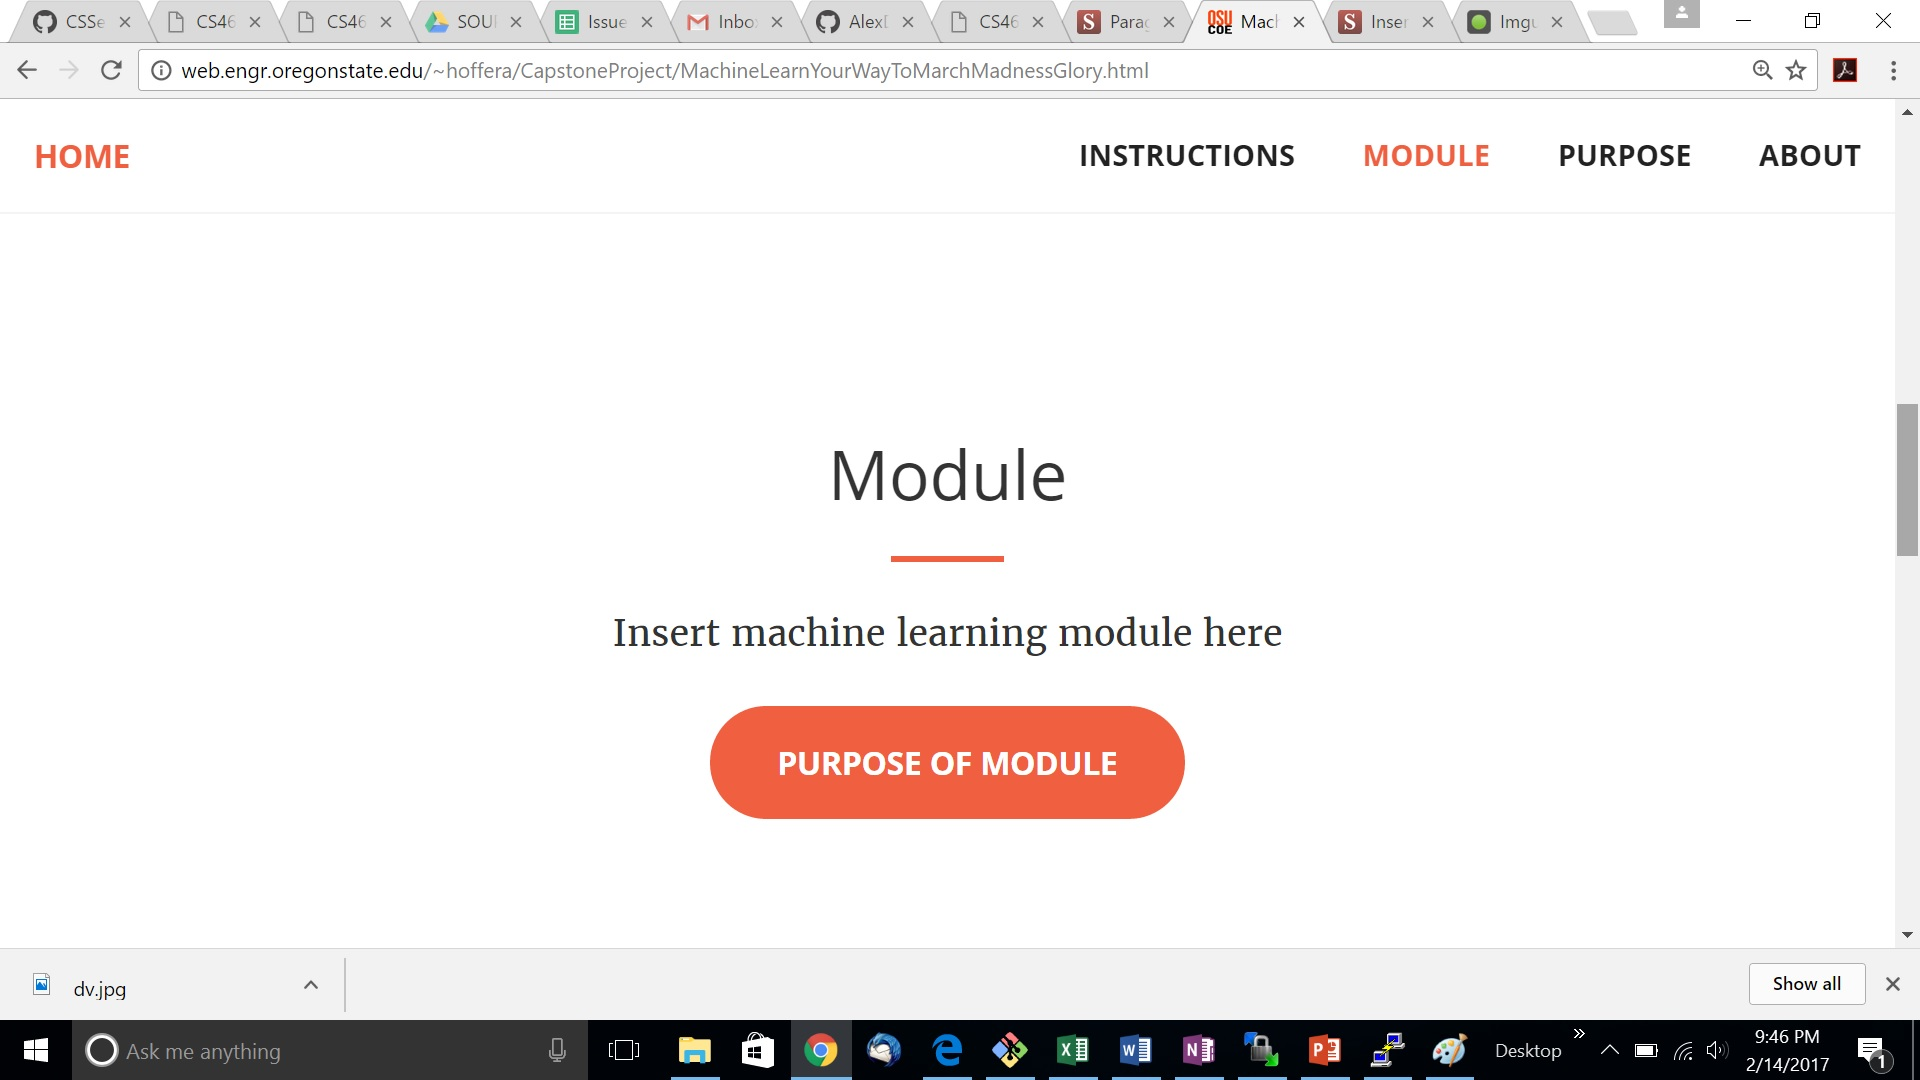
\includegraphics[width=\textwidth]{Module.jpg}
A screenshot image of the Module page. It awaits the completion of Chongxian's machine learning routines.

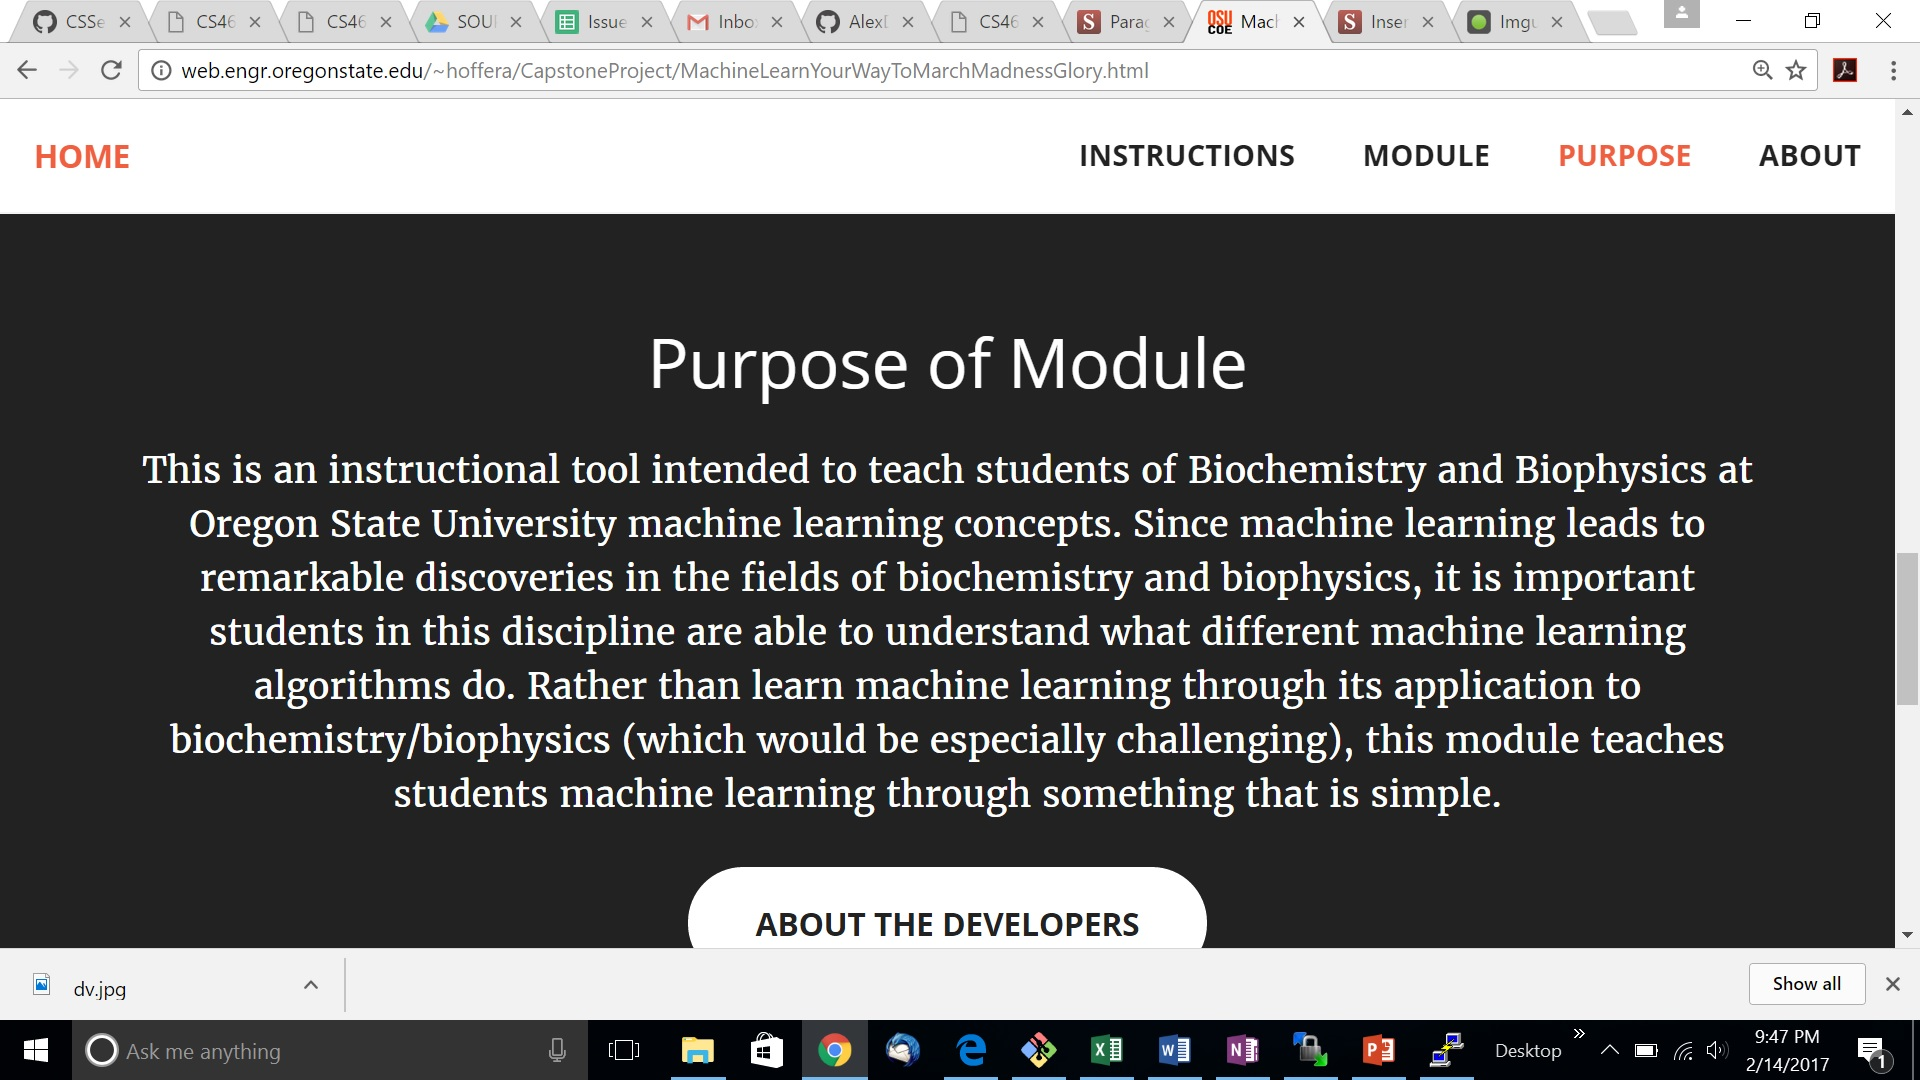
\includegraphics[width=\textwidth]{Purpose.jpg}
A screenshot image of the Purpose page, which describes why we are pursuing this project.

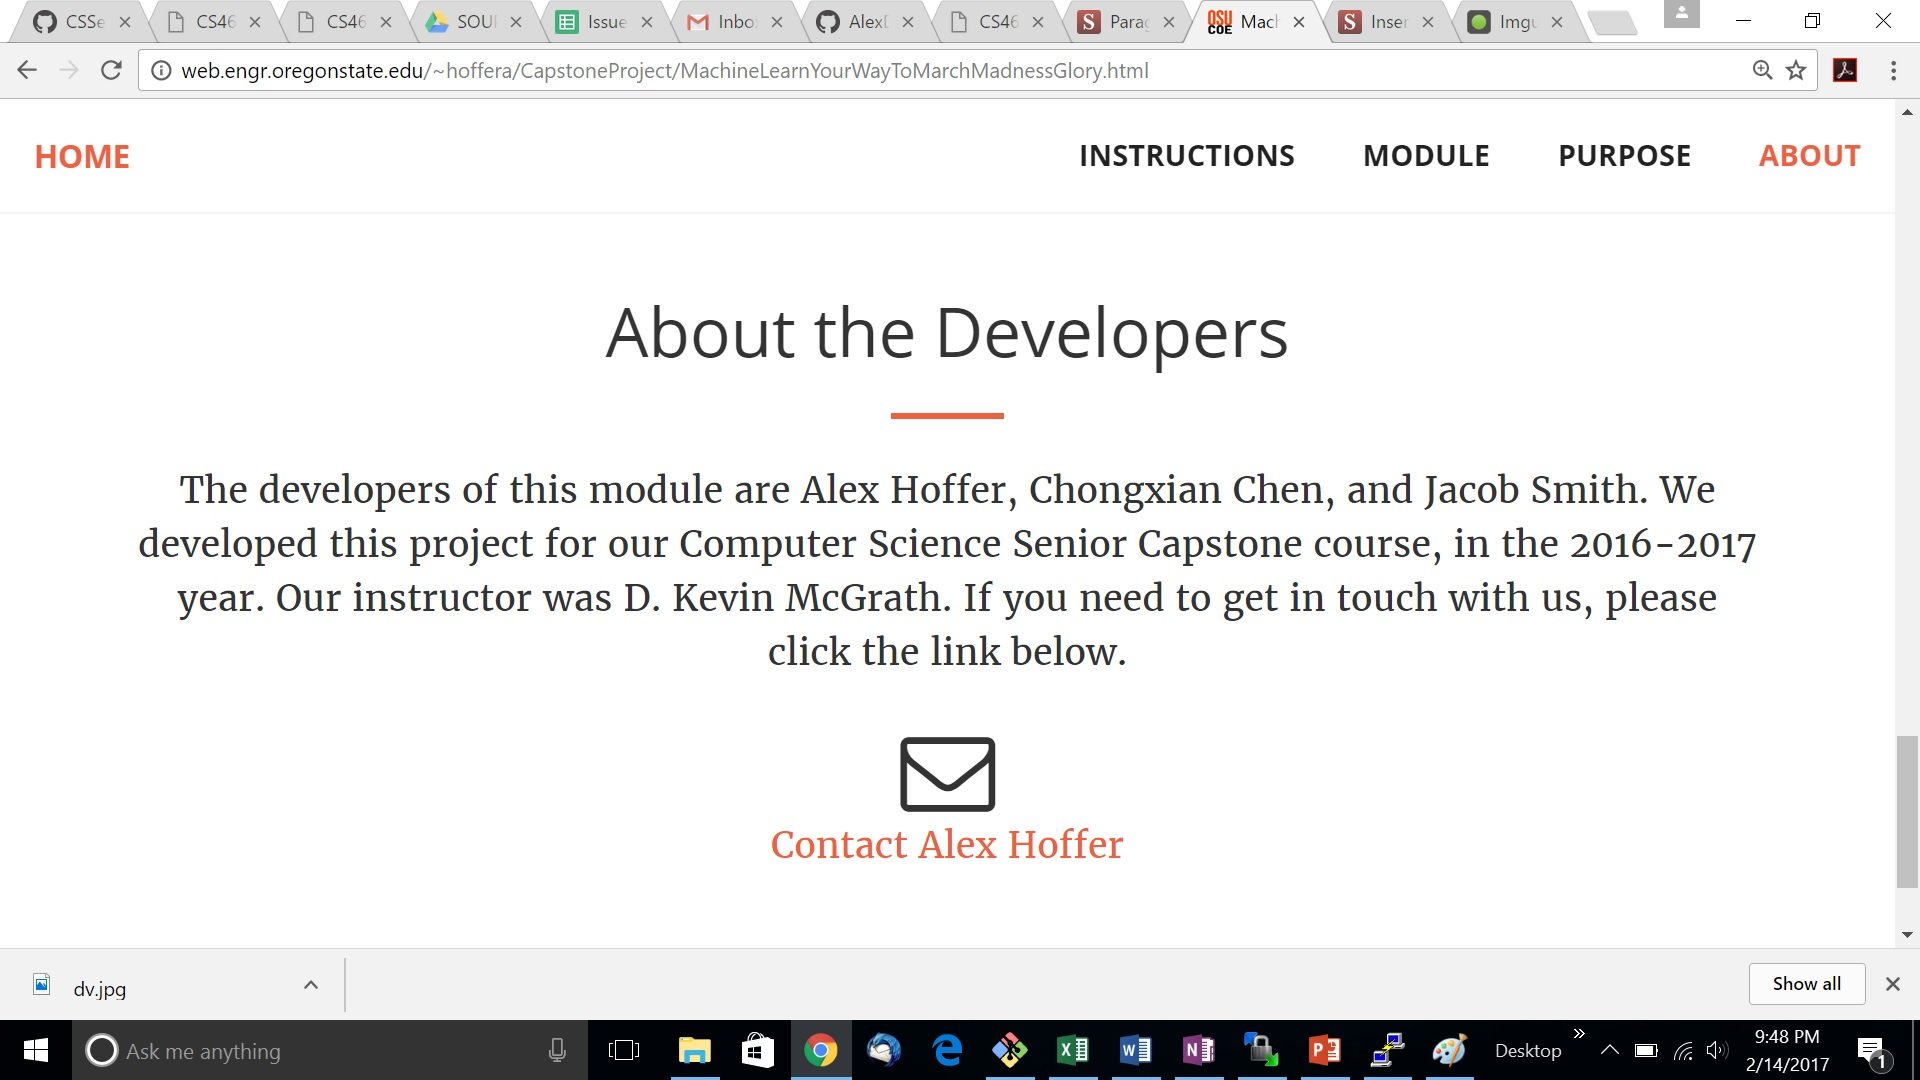
\includegraphics[width=\textwidth]{About.jpg}
A screenshot image of the About page, which describes who we are.

\subsubsection{Where Alex is currently at in the project}
\par I have two out of my three responsibilities completed, with my third contingent upon the fulfillment of my partners' responsibilities. Once we have a machine learning module, I can begin developing a data presentation feature to produce a bracket. Once this responsibility is completed, we should be done with the project.

\subsection{Chongxian Chen}

\subsubsection{Brief recap of Chongxian's responsibilities}
\par As a team, we discussed each of our three responsibilities in Fall term 2016 and documented in the design document. My three responsibilities center around Machine Learning Algorithms. I am responsible for using the data Jake collected and feed into our machine learning algorithm to train our model, then predict a basketball match results based on the data and our model. This is the responsibility 6 in our design document. My second responsibility includes moving our computing platform to a cloud platform. Potentially Amazon Web Service. This is the responsibility 7 in our design document. My third responsibility is exploring relationship between different attributes of our data and finds mathematical relationship in our prediction output. This responsibility includes the educational aspect of our project so that the biochemistry and biophysics students our client targeting can understand more about machine learning. This is the responsibility 8 in our design document.
   
\subsubsection{Responsibility 6}
\par My first responsibility is to explore machine learning, write the codes for our machine learning model and make predictions of basketball matches. As none of our members have experience with machine learning, we first get advice from our TA. Our team agrees that Python will be a powerful and convenient platform to write our code. And our TA suggested that Scikit-Learn library in Python is a great library for machine learning. Then I looked into Scikit-Learn. Scikit-Learn is an open source project licensed under the 3-Clause BSD. I found their source code on GitHub. This library is updated almost daily and stays highly active recently. There are more than 20000 commits and more than 785 contributors. I concluded that Scikit-Learn will be a reliable library for our project to do machine learning. Then I look into Scikit-Learn website and and match our project details with the examples. I found that among different categories of machine learning, our project falls into supervised leaning. More specifically, it is a supervised learning classification problem. I start from classification examples and then I also found great examples on other GitHub Repo. I also learned that I should separate the data into training data and testing data. The training data, as the name indicates, is for training our model so it can make classification predictions. The testing data, on the other hand, can provides us an overview of how accurate our model is by comparing the predictions with the testing data. Since we know the testing data is true, we can revise our model if we found our model doesn't match the truth well. Besides learning examples online, I also try to learn from Stanford Machine Learning class by Professor Andrew Ng. It's a very helpful resource also recommended by many people. It makes me understand more about the background of machine learning, what machine learning can do and how machine learning makes predictions based on data. So far, I have make predictions using Scikit-Learn. I adhere a screen shot here. The output file has two attributes. The first one has the season, team one ID, team two ID separated by an underscore. The second attribute indicate the chances the first team winning over the second team predict by our machine learning model. 

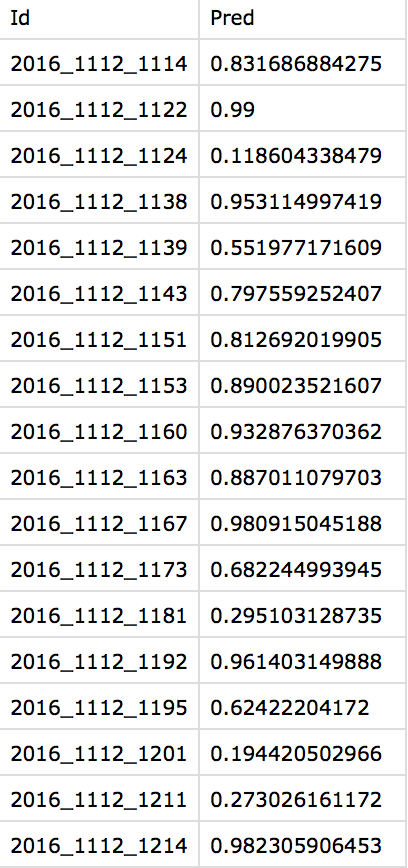
\includegraphics[width=\textwidth]{prediction.jpg}
A screenshot image of the predictions of team match results generated by our model. 

\subsubsection{Where Chongxian is currently at in the project}
\par I have one out of my three responsibilities completed. This is the most difficult part of my responsibilities. After our alpha release, I will be working on revising the output so it is more reasonable(responsibility 8). And working on allowing our users to enable and disable some attributes our data. Besides I will be working on moving our computational model to cloud.(responsibility 7). 

\subsection{Jake Smith}
\subsubsection{Responsibility 1}
My first job is to gather all the statistical data I can about Men’s NCAA basketball for both this season and previous seasons. This will be used to train and test our machine learning algorithm that will then produce a probability of one team winning over the other. I tried to gather as much data as possible, I have past season data all the way back to 1985 and all previous tournament data as well. This data did not come from any of the sites I mentioned in my tech review because the site I planned to use went from free to a pay subscription within the time I wrote the tech review to when I tried to collect the data. I found the data on a website called kaggle.com which is a data science website with a ton of data sets from every possible category or event. For this seasons data I initially started out writing a python script to scrape the data for me but am still struggling to get it to work correctly so I have been manually pulling the data from sites like espn and ncaa.com. This season won’t finish up until next term so it won’t be until next term when we can finalize our learning algorithm.
\subsubsection{Responsibility 2}
My second job is to create a database to store the data. I’ll still be using phpmyadmin for this because I have experience with it and it’s easy to use. All the data we have is in a correct format for transferring to the database, the files are either CSV or excel. Once the data is in the database I will then connect it to Alex’s webpage and display the data on the page for users to select from.
\subsubsection{Remaining Responsibilities}
I still need to finish collecting this season data which like I mentioned earlier will not be over until early next term. For doing this I am currently just pulling the data manually every week and adding it to the excel or CSV files. Next I will put all the data in the database and connect it to the webpage. After that is finished I will help Alex display the python module on the page and test it. Also I will be helping George with his training and testing sets to include the most influential data.

\end{document}